\documentclass[tikz,border=14pt]{standalone}
\usepackage{tikz}
\begin{document}
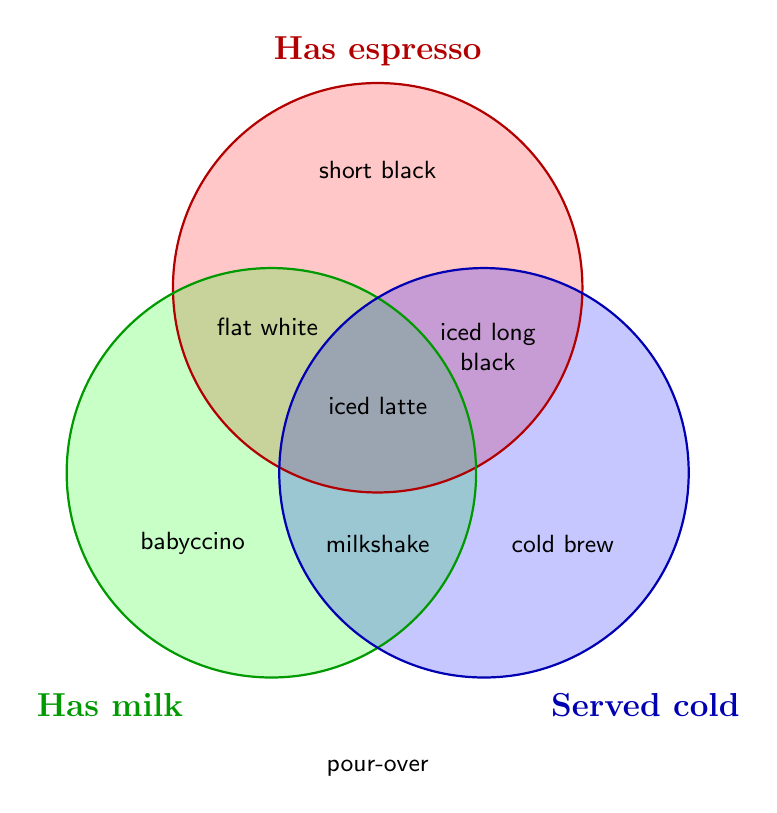
\begin{tikzpicture}[font=\sffamily\small]

  % Circle geometry
  \def\r{2.6}
  \coordinate (A) at (0, 1.5);      % Has espresso
  \coordinate (B) at (-1.35, -0.85); % Has milk
  \coordinate (C) at (1.35, -0.85);  % Served cold

  % Fills
  \begin{scope}
    \fill[red, opacity=0.22]   (A) circle (\r);
    \fill[green, opacity=0.22] (B) circle (\r);
    \fill[blue, opacity=0.22]  (C) circle (\r);
  \end{scope}

  % Outlines
  \draw[thick, red!70!black]   (A) circle (\r);
  \draw[thick, green!60!black] (B) circle (\r);
  \draw[thick, blue!70!black]  (C) circle (\r);

  % Circle titles
  \node[font=\bfseries\large, red!70!black]   at (0, 4.5)      {Has espresso};
  \node[font=\bfseries\large, green!60!black] at (-3.4, -3.8)  {Has milk};
  \node[font=\bfseries\large, blue!70!black]  at (3.4, -3.8)   {Served cold};

  % Drink labels in their regions
  \node[align=center] at (0, 3.0)     {short black};        % espresso only
  \node[align=center] at (-1.4, 1.0)  {flat white};         % espresso + milk
  \node[align=center] at (1.4, 0.75)  {iced long\\black};   % espresso + cold
  \node[align=center] at (0, 0.0)     {iced latte};         % all three
  \node[align=center] at (-2.35, -1.75) {babyccino};        % milk only
  \node[align=center] at (0, -1.75)   {milkshake};          % milk + cold
  \node[align=center] at (2.35, -1.75) {cold brew};         % cold only
  \node[align=center] at (0, -4.6)    {pour-over};          % outside all three

\end{tikzpicture}
\end{document}